%conceitos básicos deviam ser mais abstratos, e não falar a respeito de características da placa/processador físico.

\chapter{EPOS}

%alarm's diagram
%alarm's queue

%scheduling

%Processo de inicialização do epos (crt, inits, etc).
%explicar crts... (good luck on that my boy).
%falar talvez do estilo do código (_asdf é private, etc).
%epos mote

%cite some works that used EPOS (specially giovani's).


%source: http://epos.lisha.ufsc.br/EPOS+User+Guide
EPOS (Embedded Parallel Operating System) é um sistema operacional orientado a aplicação, cujo design chama-se ADESD (\emph{Application-Driven Embedded System Design Method}), proposto por Fröhlich \cite{guto_thesis}. A ideia central do EPOS é prover um sistema operacional mínimo, de modo a minimizar o \emph{overhead} da existência de um sistema operacional, deixando o processador livre para executar a aplicação do desenvolvedor \cite{epos_user_guide}.

Como o objetivo é criar um ambiente em que o desenvolvedor possa rapidamente produzir suas aplicações, EPOS provê vários utilitários comumente usados em aplicações, como filas, listas, tabelas de hashs, vetores, semáforos, OStream (para imprimir na tela), números aleatórios, cálculo de CRC e etc. Além destes utilitários, EPOS também provê uma série de componentes como threads, alarmes, cronometros, \emph{heaps} e meios para acessar a rede (internet).

\section{Arquitetura do EPOS}


\textbf{Linguagem e paradigma:} O EPOS é escrito em C++, e não em C, como é tradicionalmente feito. Como paradigma, é usado orientação à objetos, então cada componente do EPOS está encapsulado por uma classe (como a heap, timer, thread, etc). No EPOS também é muito usado conceitos como herança e metaprogramação estática (que será abordado mais a frente).

\textbf{Mediadores de Hardware:} Dentro da arquitetura do EPOS há o conceito de mediadores de hardware, que são os componentes (ou classes) dependentes de plataforma. Idealmente, as únicas classes que precisam ser modificadas e/ou reimplementadas são os mediadores. Há mediadores específicos da placa, como por exemplo Pandaboard, Zedboard e etc; abstraídos sob o nome de \emph{machine} e mediadores específicos de um processador, abstraídos sob o nome de \emph{architecture}. No código do EPOS, estes mediadores encontram-se nas pastas \emph{mach} e \emph{arch}.
% Fonte: Hardware Mediators: A Portability Artifact for Component-based Systems
% HAL vs Virtualização vs Mediadores

Mediadores de hardware são uma alternativa ao tradicional uso de VMs\footnote{Virtual Machines.} e de HAL\footnote{Hardware Abstraction Layer}, proposta por Fröhlich em seu trabalho \emph{Application-Oriented System Design} \cite{guto_thesis}. O problema do uso de VMs é o seu \emph{overhead} causado devido à tradução das operações da VM em código nativo. Já o uso de um HAL incorre no problema da manutenibilidade e dificuldade de adapção à novas arquiteturas muito distintas entre si \cite{hw_mediators}. O HAL não conseguiu passar pela ``prova do tempo'', e já está sendo considerado obsoleto por distribuições GNU/Linux populares, como o 
Ubuntu\footnote{\url{http://www.linux-magazine.com/Online/News/Ubuntu-10.04-Alpha-2-Removes-HAL}}, sendo chamado de ``uma grande não-manutenível bagunça monolítica''\footnote{\url{https://wiki.ubuntu.com/Halsectomy}}.

%\textbf{Traits:} Traits são classes onde é possível configurar certos componentes do EPOS em tempo de compilação. Lá é possível, por exemplo, definir o tamanho da \emph{stack} e \emph{heap} do sistema, a sua frequência de \emph{clock} bem como ativar ou desativar certas funções do sistema. Esta classe normalmente precisa ser alterada em um porte, mesmo ela não sendo um mediador de hardware, pois eles usam as configurações descritas nos traits.

\textbf{Interface Infladas: } Um conceito importante da arquitetura do EPOS é a Interface Inflada. %http://www.inf.ufsc.br/~guto/publications/aoos.pdf
Em sistemas orientados a aplicação, famílias de abstrações são frequentemente tratadas como entidades únicas, algo que pode ser vantajoso para o programador da aplicação, já que este não precisaria se preocupar com qual membro em específico desta família ele precisaria usar \cite{guto_thesis}.

Interface inflada basicamente é uma interface que declara os métodos de todas as classes que derivam dela, exportanto assim todos os métodos daquela família de abstrações, como mostra a figura \ref{fig:inflated}. Deste modo, o desenvolvedor de aplicativo poderia escrever a aplicação inteira em termos da interface inflada, relegando a tarefa de configuração do sistema a um utilitário automatizado. Tal utilitário poderia, através de uma análise sintática do código fonte, escolher quais os membros mais apropriados da família exportada serão associados no momento da compilação \cite[p.~56]{guto_thesis}.

%write about specifics from timers
\begin{figure}[ht!]
	\label{fig:inflated}
    \centering
    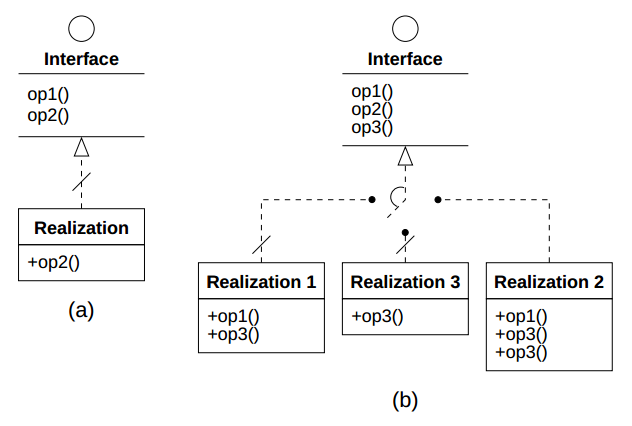
\includegraphics[width=7.5cm]{figuras/inflated_interface}
    \caption{Exemplos de uso de interfaces infladas \cite{guto_thesis}.}
\end{figure}


%%%%%


\section{Modos de Compilação}


\section{Traits}

Existem 4 arquivos traits.h que devem ser levados em consideração em um porte, dois deles devem ser completamente reescritos. Os arquivos \verb+./include/traits.h+ e \verb+/include/system/traits.h+ (onde `.' é a pasta raiz do código) possuem configurações gerais do EPOS, que, a princípio, devem ser independentes de arquitetura. Na prática há alguns pequenos ajustes que devem ser feitos nesses arquivos, pois é lá que se define, por exemplo, se o EPOS trabalhará em um processador \emph{multicore}, se utilizará \emph{scratchpad}, quais componentes estarão em modo de depuração e etc; entretanto isto se resume a trocar o valor de algumas variáveis de \emph{true} para \emph{false} e vice-versa.

Os outros dois arquivos são \verb+./include/mach/zynq/traits.h+ e\\ \verb+./include/arch/armv7/traits.h+. Essa divisão é necessária pois, como dito anteriormente, é possível de um mesmo processador estar em diferentes \emph{machines}, e, caso seja necessário fazer um porte para aquela plataforma, bastaria modificar os arquivos da pasta \emph{mach}, deixando os da pasta \emph{arch} praticamente intactos, o que facilita muito novos portes.

O arquivo \verb+./include/arch/armv7/traits.h+ trata das opções específicas do processador, portanto é lá que opções como \emph{endianess}, velocidade de \emph{clock}, número de \emph{cores}, tamanho da \emph{heap} e \emph{stacks}, bem como outras opções pertinentes ao mapeamento de memória e opções da MMU podem ser configuradas.

No arquivo de traits da \emph{machine}, ficam as opções de configuração de componentes como a UART, controlador de interrupções, \emph{timer}, e qualquer componente de interfaceamento externo à placa (rede, por exemplo). Componentes podem ser facilmente ativados ou desativados nestas opções.

\section{Interrupções}


Como o EPOS foca do desempenho da aplicação, em seu design opta-se por utilizar a menor quantidade possível de interrupções, e evitá-las sempre que possível, isto contribui também para que o sistema seja mais previsível. Se a aplicação não precisar de componentes específicos que necessitem interrupções (como um rádio, por exemplo), a única interrupção a ser tratada será a do \emph{timer}, já que o escalonador e alarm necessitam dele.

%interrupções (indexação de um vetor de interrupções pelo seu ID)
%exception -> ic_handler -> timer_handler -> alarm handler
%                                         -> scheduelr handler

A sequência de chamadas de função, dado o recebimento de uma interrupção de \emph{timer} está ilutrada na figura \ref{fig:exception_handling}. Exception é um código em assembly cujo objetivo é salvar o contexto no recebimento da chamada, chamar o tratador de interrupções padrão, e restaurar o contexto após isto. O tratador de interrupções do \emph{interrupt controller} (IC) possui um vetor de tratadores de interrupção, onde para cada número de interrupção, há uma entrada correspondente no vetor. Este tratador então lê o registrador responsável por armazenar o número da interrupção gerada (esta parte é dependente de arquitetura, na Zedboard uma interrupção de timer tem número 29, por exemplo), indexa seu vetor e chama o tratador apropriado. Chegando no tratador do \emph{timer}, este chama os tratadores de todos os componentes que dependem de um \emph{timer}, neste caso o \verb+Alarm+ e \verb+Scheduler+.

\fig{0.18}{exception_handling}{Sequência de chamada de tratadores de interrupção. A interrupção gerada neste exemplo foi uma de \emph{timer}}. 



\section{Gerenciamento de Memória}

Uma das principais funções de um sistema operacional é o gerenciamento de memória. Isto inclui organizar a memória (mapeamento de memória, definição do que cada região da memória guarda, etc) e gerenciamento (manter registro de páginas livres, definir permissões, etc).

% MMU::alloc

Para entendermos como isto é feito, primeiro é necessário entendermos como funciona a abstração da MMU no EPOS. Isto se dá com 4 classes principais, a \verb+ARMv7_MMU+, que possui a lista de memória livre, a \verb+Page_Table+, que mapeia porções de até 1MB de endereço virtual para físico, \verb+Chunk+, que nada mais é que um conjunto de \verb+Page_Tables+, e, finalmente, \verb+Directory+, que é um conjunto de \verb+Chunks+ (ou \verb+Page_Tables+).

A classe \verb+ARMv7_MMU+ possui uma uma lista de porções de memória livre, gerenciadas pelas funções \verb+alloc+ e \verb+free+. A granularidade destas porções de memória é a de um \emph{frames}
\footnote{Frame é uma porção de tamanho fixo de memória física (normalmente 4KB). A diferença entre uma página e um frame é que um frame referece à uma porção da memória física, enquanto uma página referece à uma porção de memória virtual.}.
Note que esta lista utiliza os endereços \textbf{físicos} destas porções de memória.

A tabela de páginas da MMU do ARMv7, assim como a do IA32, possui dois níveis. Na nomenclatura da ARM, a tabela de nível mais alto é a tabela L1 (de \emph{level}), onde cada entrada desta tabela aponta para outra tabela (uma tabela L2).
Cada entrada da tabela L2 possui o endereço físico correspondente ao endereço virtual requisistado. A maneira como esta tabela é usada para traduzir um endereço virtual para um físico varia de arquitetura para arquitetura, sendo esta parte explicada detalhadamente na seção \ref{sec:mmu}.

Nas abstrações do EPOS, a classe que gerencia a tabela L2 é a \verb+Page_Table+, e a classe que gerencia a tabela L1 é a \verb+Directory+. Portanto uma \verb+Page_Table+ é apenas um vetor, onde em cada posição está escrita uma posição de memória física, junto de algumas \emph{flags} (que definem permissões, ``cacheabilidade'' e etc). O número máximo de entradas numa \verb+Page_Table+ é dependente de arquitetura. No ARMv7 são 256 entradas de 4 bytes (mapeando até 1MB de memória portanto), e no IA32 são 1024 entradas (que mapeiam até 4MB).

\verb+Chunk+ é uma classe bastante importante, e, apesar de simples, é importante que se tenha um bom entendimento sobre como ela funciona.
Cria-se um chunk para alocar uma certa porção de memória, em um espaço de endereçamento próprio. 

Esta classe recebe dois parâmetros: A quantidade de bytes a serem alocados, e as \emph{flags} a serem usadas. \verb+Chunk+ então calcula quantas tabelas de páginas serão necessárias para mapear a quantidade de bytes requisitada, e então cria estas páginas contiguamente (em qualquer lugar da memória, a ser decidido pela função \verb+alloc+).

\verb+Chunk+ então chama a função \verb+map+ de \verb+Page_Table+ para mapear aquela porção da memória. Cada \emph{frame} é requisitado pela função \verb+alloc+, o que significa que cada \verb+Page_Table+ pode estar apontando para qualquer posição da memória, não estando os \emph{frames} necessariamente contiguos na memória física, apesar que eles serão \textbf{contíguos} no espaço de memória virtual mapeada num mesmo \verb+Chunk+.

Portanto esta classe efetivamente aloca uma porção de memória em um espaço de endereçamento próprio, este fato será bastante importante quando discutirmos a criação das heaps de usuário e do sistema.

%Directory

Já a classe directory é responsável por gerenciar e unificar todas estas porções de memória. Sua principal função é a \verb+attach+, que tomando como parâmetro um \verb+Chunk+, mapeia cada uma de suas páginas contiguamente (isto é, cria uma entrada em directory que a aponta para uma página criada em \verb+Chunk+, para cada página).

A figura \ref{fig:mmu_translation} ilustra a interação entre os conteúdos das entradas de \verb+Directory+ e \verb+Page_Table+ com a memória física. A quantidade de bits usada para indexar as tabelas é dependente de arquitetura. Aqui, os primeiros 12 bits indexam a tabela de \verb+Directory+, os 8 bits seguintes indexam a tabela de \verb+Page_Table+, e os últimos 12 bits são simplesmente copiados do endereço virtual para o físico. Mais detalhes sobre este processo na seção \ref{sec:mmu}, em particular na imagem \ref{fig:translation}.

%\fig{0.42}{mmu_translation}{Interação entre \verb+Directory+ e \verb+Page_Table+ com a memória física.}


\fig{0.22}{mmu_translation}{Interação entre Directory e Page\_Table com a memória física. Neste exemplo, o endereço virtual 0xAB2FF1234 seria traduzido para o endereço físico 0xDEAD11234. A última posição de memória física indexável neste exemplo é 0x1FFFF\_\_\_ pois a Zedboard dispõe de 512MB.}

\verb+Directory+ não sabe a qual \verb+Chunk+ uma determinada \verb+Page_Table+ pertence, e a tradução de endereços pode ocorrer independente desta informação. Na figura \ref{fig:mmu} é ilustrada a interação entre as classes discutidas.

\fig{0.42}{mmu}{Diagrama de classes da MMU.}


%make a diagram showing how MMU alloc a physical page, and how the heap lends pages that were already allocated in the MMU's point of view.

\subsection{Heaps}

A heap é responsável por armazenar e gerenciar os dados dinâmicos criados durante a execução da aplicação (a cada \verb+malloc/new+ executado, por exemplo). Existe duas heaps: A do sistema, e a do usuário. É possível compilar o EPOS com apenas a heap do sistema, quando o desenvolvedor decide que a aplicação deverá rodar em modo privilegiado, não sendo usado portanto o modo usuário (isto é configurável nos \verb+traits+).

A memória da heap é alocada através de um \verb+Chunk+. É neste ponto que pode-se atribuir flags que limitam as permições de acesso (a heap de usuário é alocada sem restrições de acesso, já a do sistema aloca uma porção de memória que só pode ser acessada em modo privilegiado). É por usar um \verb+Chunk+ também que do ponto de vista da aplicação, é como se ela tivesse acesso à todo o espaço de memória. Note que do ponto de vista da MMU (e sua lista de memória livre), é como se a porção de memória da heap estivesse em uso, já a heap vê sua porção de memória como livre.

A heap trabalhada com uma lista de memória livre (igual à da MMU), só que ao contrário da MMU, que aloca somente páginas (frames) inteiras de memória, a heap aloca quantidades de memória com a granularidade de bytes.

Para que a heap do sistema e a heap do usuário seja corretamente usada, faz-se no EPOS \emph{overload} do operador \verb+new+ e \verb+delete+, e \emph{placement new}. Por exemplo, um \verb+new A()+ chamaria a seguinte sequencia de funções:

\begin{verbatim}
inline void * operator new(size_t bytes) {
    return malloc(bytes);
}
inline void * malloc(size_t bytes) {
    if(Traits<System>::multiheap)
        return Application::_heap->alloc(bytes);
    else
        return System::_heap->alloc(bytes);
}
\end{verbatim}

O compilador se encarrega de avaliar o \verb+sizeof+ de \verb+A+, e envia como parâmetro para o operador \verb+new+. \verb+multiheap+ é um atributo dos traits que define se o sistema possui uma heap de usuário separada da do sistema ou se é usada somente uma única heap.

Para o sistema alocar memória usando sua própria heap com o operador \verb+new+, faz-se um \emph{overload} do \emph{placement new}, como segue:

\begin{verbatim}
enum System_Allocator {SYSTEM};

inline void * operator new(size_t bytes, const EPOS::System_Allocator & allocator) {
    return EPOS::System::_heap->alloc(bytes);
}
\end{verbatim}

Feito isto, para alocar, dentro do EPOS, alguma porção de memória utilizando o operador \verb+new+ com a heap do sistema, basta escrever \verb+(SYSTEM)+ logo após o \verb+new+, por exemplo:

\begin{verbatim}
_timer = new (SYSTEM) Alarm_Timer(handler);
\end{verbatim}


\section{Escalonadores}

%falar dos escalonadores que o EPOS suporta
%falar do gio <3



















